\documentclass[../../InformazioneQuantistica.tex]{subfiles}
\begin{document}

\chapter{Complementi}
\marginpar{Fonti utili: \cite{Fermi-rule}, \cite{MIT-Time}}
\section{Teoria delle perturbazioni dipendenti\\ dal tempo}
\lesson{17}{12/6/2019}
Consideriamo un sistema quantistico - che può essere costituito da atomi, o più in generale da qubit - e che vogliamo poter regolare dall'esterno, per esempio mediante impulsi di radiazione elettromagnetica. Vogliamo poter descrivere cosa accada agli stati quantistici a seguito di un potenziale che \textit{varia nel tempo}. Dal punto di vista energetico, alcune delle possibili conseguenze di una perturbazione sono date da:
\begin{itemize}
\item \textbf{Assorbimento} dell'energia della perturbazione, con passaggio tra stati $\ket{i} \to \ket{f}$, con $\mathcal{E}_i < \mathcal{E}_f$
\item \textbf{Emissione} di parte dell'energia contenuta nello stato, con passaggio tra stati $\ket{i}\to \ket{f}$ con $\mathcal{E}_i > \mathcal{E}_f$
\item Passaggio da un autovalore dell'energia nello spettro \textit{discreto} a uno dello spettro \textit{continuo}.
\end{itemize}

Nello specifico, supponiamo che il sistema sia descritto da un'Hamiltoniana $H(t)$ scomponibile in un termine $H_0$ indipendente da $t$, e un potenziale $W(t)$ che invece dipende da $t$:
\begin{align*}
    H(t) = H_0 + \lambda W(t)
\end{align*}
dove $\lambda$ è un parametro che quantifica \textit{il rapporto} tra le due componenti $H_0$ e $W(t)$.\\
Denotiamo con $\ket{\varphi_n}$ gli autostati di $H_0$ (che supponiamo avere solo spettro discreto) di autovalore $\mathcal{E}_n$, che consideriamo conosciuti:
\begin{align*}
    H_0\ket{\varphi_n} = \mathcal{E}_n \ket{\varphi_n}
\end{align*}
Per $\lambda = 0$ l'evoluzione temporale dipende solo da $H_0$, ossia da un potenziale costante. In tal caso, se il sistema si trova in un autostato $\ket{\varphi_n}$ di $H_0$ a $t=0$, allora è nello stesso autostato a qualsiasi altro istante (e infatti $\ket{\varphi_n}$ sono detti \textbf{stati stazionari}). In particolare, la probabilità che il sistema nello stato $\ket{\psi(t=0)} = \ket{\varphi_i}$ si trovi in $\ket{\varphi_f}$ ad un istante $t$ è esattamente nulla:
\begin{align*}
    P_{if}^0(t) = |\braket{\varphi_f|\psi(t)}|^2 = \left|\braket{\varphi_f|\varphi_i} \exp\left(-\frac{i}{\hbar}t \mathcal{E}_f\right) \right|^2 \equiv 0
\end{align*}
Tale $P_{if}(t)$ non è altro che la \textbf{probabilità di transizione} tra l'evoluzione temporale di $\ket{\varphi_i}$ al tempo $t$ e $\ket{\varphi_f}$.\\

Se $\lambda \neq 0$, in generale, $P_{if}(t) \neq 0$. In altre parole, la presenza di un potenziale che varia nel tempo fa sì che quelli che prima erano stati stazionari ora non lo siano più.\\
Cerchiamo quindi un modo per calcolare tale $P_{if}(t)$ nel caso generale. Nella visuale di Schr\"odinger, l'evoluzione temporale di uno stato è data dall'equazione di Schr\"odinger dipendente dal tempo:
\begin{align}
    i\hbar \frac{d}{dt} \ket{\psi(t)} = \Big[H_0 + \lambda W(t) \Big] \ket{\psi(t)}
    \label{eqn:schrodinger-dip-t}
\end{align}
Basta allora trovare la $\ket{\psi(t)}$ che risolve tale equazione con la condizione iniziale $\ket{\psi(t=0)} = \ket{\varphi_i}$, e si può calcolare la probabilità desiderata:
\begin{align*}
    P_{if}(t) = |\braket{\varphi_f|\psi(t)}|^2
\end{align*}
Per farlo, riscriviamo la (\ref{eqn:schrodinger-dip-t}) in coordinate, scegliendo come base quella formata dagli autostati di $H_0$. Partiamo trasformando la $\ket{\psi(t)}$:
\begin{align}
    \ket{\psi(t)} = \bb{I}\ket{\psi(t)} \underset{(a)}{=} \sum_{k=0}^{+\infty}\underbrace{\braket{\varphi_n|\psi(t)}}_{c_n(t)}\ket{\varphi_n} = \sum_{k=0}^{+\infty} c_n(t) \ket{\varphi_n}
    \label{eqn:psi-t-baseH0}
\end{align}
dove in (a) si è usata la completezza di Dirac. Sostituendo in (\ref{eqn:schrodinger-dip-t}) si ottiene:
\begin{align*}
    i\hbar \frac{d}{dt} \sum_{k=0}^{+\infty} c_k(t) \ket{\varphi_k} = H_0 \sum_{k=0}^{+\infty} c_k(t)\ket{\varphi_n} + \lambda W(t) \sum_{k=0}^{+\infty} c_k(t) \ket{\varphi_k}
\end{align*}
Prendiamo il prodotto scalare con $\ket{\varphi_n}$:
\begin{align*}
    i\hbar \frac{d}{dt} \sum_{k=0}^{+\infty} c_k(t) \underbrace{\braket{\varphi_n|\varphi_k}}_{\delta_{nk}} = \sum_{k=0}^{+\infty} c_k(t) \underbrace{\bra{\varphi_n}H_0 \ket{\varphi_k}}_{\delta_{nk}\mathcal{E}_k} + \lambda \sum_{k=0}^{+\infty} c_k(t) \underbrace{\bra{\varphi_n}W(t)\ket{\varphi_k}}_{W_{nk}(t)}
\end{align*}
Giungiamo allora al sistema di equazioni:
\begin{align}
    i\hbar \dot{c}_n(t) = \mathcal{E}_n c_n(t) + \lambda \sum_{k=0}^{+\infty} W_{nk}(t) c_k(t)
    \label{eqn:equazioni-dip-t}
\end{align}
Poiché in generale $W(t)$ non è diagonale in questa base, le equazioni differenziali sono \textit{accoppiate} tra loro, e perciò risultano di difficile soluzione.\\

\begin{comment}
Nello specifico, vogliamo risolvere l'equazione di Schr\"odinger dipendente dal tempo:
\begin{align*}
i \hbar \frac{d}{dt}\ket{\psi(t)} = [H_0 + \lambda W(t) ] \ket{\psi(t)}
\end{align*}
Lavoriamo nell'ipotesi di \textit{perturbazione piccola} ($\lambda \ll 1$), e di conoscere gli autovalori e gli autostati del caso imperturbato, che ipotizziamo essere appartenenti al solo spettro discreto:
\begin{align*}
H_0 \ket{\varphi_n} =\mathcal{E}_n \ket{\varphi_n}
\end{align*}
Consideriamo uno stato iniziale $\ket{\psi(t=0)}=\ket{\varphi_i}$ pari ad un autostato di $H_0$. Ci interessano le probabilità di transizione ad uno stato finale $\ket{\varphi_f}$ date da:
\begin{align*}
P_{if}(t) = |\braket{\varphi_f | \psi(t)}|^2
\end{align*}
Partiamo allora  scrivendo la funzione d'onda all'istante $t$ nella base degli autostati di $H_0$:
\begin{align*}
\ket{\psi(t)} = \sum_{n=1}^{+\infty} c_{n}(t) \ket{\varphi_n}; \qquad c_n(t) = \braket{\varphi_n|\psi(t)}
\end{align*}
Possiamo calcolare gli elementi di matrice del potenziale di perturbazione:
\begin{align*}
\bra{\varphi_n} W(t) \ket{\varphi_k} = W_{nk}(t)
\end{align*}
In questa base $H_0$ è ovviamente diagonale:
\begin{align*}
\bra{\varphi_n}H_0 \ket{\varphi_k} = \mathcal{E}_n \delta_{nk}
\end{align*}
Così facendo, possiamo proiettare l'equazione di Scr\"odinger su questa base, ottenendo un'equazione differenziale che coinvolge gli elementi di matrice:
\begin{align*}
i\hbar \frac{d}{dt}c_n(t) = \mathcal{E}_n c_n(t) + \sum_k \lambda W_{nk} c_k(t)
\end{align*}
\end{comment}

Cerchiamo allora di semplificare il problema. Partiamo passando in visuale di interazione, ponendo:
\begin{align}
    \ket{\psi(t)}_I = \exp\left(\frac{i}{\hbar} t H_0 \right) \ket{\psi(t)}_S
    \label{eqn:visuale-interazione}
\end{align}
dove $\ket{\psi(t)}_S$ è la funzione d'onda nella visuale di Schr\"odinger (finora utilizzata).\\
Nel caso di (\ref{eqn:psi-t-baseH0}), otteniamo:
\begin{align*}
    \sum_{k=0}^{+\infty} b_n(t) \ket{\varphi_n} \equiv \ket{\psi(t)}_I = \sum_{k=0}^{+\infty}\exp\left(\frac{i}{\hbar}t \mathcal{E}_n\right) c_n(t) \ket{\varphi_n}
\end{align*}
Proiettando in coordinate (ossia prendendo il prodotto scalare per $\ket{\varphi_n}$), si giunge a:
\begin{align}
    b_n(t) = c_n(t) \exp\left(\frac{i}{\hbar}\mathcal{E}_nt\right) \Rightarrow c_n(t) = b_n(t)\exp\left(-\frac{i}{\hbar}\mathcal{E}_nt\right)
    \label{eqn:bn}
\end{align}
Tale manipolazione permette di semplificare notevolmente la notazione. Infatti, sostituendo (\ref{eqn:bn}) in (\ref{eqn:equazioni-dip-t}) otteniamo:
\begin{align*}
    i\hbar \left( \cancel{b_n(t) \left(-\frac{i}{\hbar} \mathcal{E}_n \right)} + \dot{b}_n(t) \right) \exp\left(-\frac{i}{\hbar} \mathcal{E}_n t\right) &= \cancel{\mathcal{E}_n b_n(t) \exp\left(-\frac{i}{\hbar}\mathcal{E}_n t \right)} +\\
    &+ \lambda \sum_{k=0}^{+\infty} W_{nk}(t) b_k(t) \exp\left(-\frac{i}{\hbar} \mathcal{E}_k t \right)
\end{align*}
e dividendo per l'$\exp$:
\begin{align}
    i\hbar \dot{b}_n(t) = \lambda \sum_{k=0}^{+\infty} W_{nk}(t) b_k(t) \exp(i\omega_{nk}t); \qquad \omega_{nk} = \frac{\mathcal{E}_n - \mathcal{E}_k}{\hbar}
    \label{eqn:equazioni-bn-dip-t}
\end{align}
Abbiamo perciò rimosso l'evoluzione data dal potenziale costante $H_0$, focalizzandoci solo sull'azione della componente dipendente dal tempo $W(t)$.\\

\begin{expl}
Geometricamente, possiamo immaginare l'evoluzione data da $H(t)$ come la sovrapposizione di due \textit{rotazioni} a diverse velocità - una costante (data da $H_0$) e una variabile (da $W(t)$). In quest'ottica, le $b_n(t)$ non sono altro che le coordinate di $\ket{\psi(t)}$ rispetto ad una base che \q{evolve come prescritto da $H_0$}, e che funge da una sorta di \q{sistema di riferimento rotante solidale alla rotazione data da $H_0$}.\\
In altre parole, nella base data da:
\begin{align*}
    \left\{ \exp\left(\frac{i}{\hbar} t \mathcal{E}_n \right) \ket{\varphi_n}\right\}_{n\in \bb{N}}
\end{align*}
l'evoluzione unitaria data dall'Hamiltoniana $H_0$ coincide con l'\textbf{identità}.
\end{expl}

Nonostante la notazione appena più semplice, le (\ref{eqn:equazioni-bn-dip-t}) sono ancora molto difficili da risolvere. Per procedere assumiamo perciò l'\textbf{ipotesi perturbativa}, per cui le $b_n(t)$ ammettono uno sviluppo in serie di potenze attorno a $\lambda=0$:
\begin{align}
b_n(t) = b_n^{(0)} (t) + \lambda b_n^{(1)}(t) + \lambda^2 b_n^{(2)}(t) + \dots
\label{eqn:serie-bn}
\end{align}
Equivalentemente, per il relativo ket vale:
\begin{align*}
    \ket{\psi(t)}_I &= (b_n^{(0)}(t) + \lambda b_n^{(1)}(t) + \dots ) \ket{\varphi_n} =\\
    &\equiv \ket{\psi^{(0)}(t)} + \lambda \ket{\psi^{(1)}(t)} + \lambda^2 \ket{\psi^{(2)}(t)} + \dots 
\end{align*}
Sostituendo (\ref{eqn:serie-bn}) in (\ref{eqn:equazioni-bn-dip-t}) giungiamo a:
\begin{align*}
    i\hbar \Big( \dot{b}_n^{(0)}(t) + \lambda \dot{b}_n^{(1)}(t) + \dots \Big) = \sum_{k=0}^{+\infty} W_{nk}(t) \Big[\lambda b_k^{(0)}(t) + \lambda^2 b_k^{(1)}(t) + \dots \Big] \exp(i\omega_{nk}t)
\end{align*}
Poiché tale equazione deve valere $\forall \lambda \in \bb{R}$, possiamo uguagliare i coefficienti delle $\lambda$ di ciascun ordine. Per $\lambda^0$ otteniamo:
\begin{align*}
    i\hbar \dot{b}_n^{(0)}(t) = 0 \Rightarrow b_n^{(0)}(t) = b_n^{(0)}(0)
\end{align*}
Imponendo la condizione iniziale ($\ket{\psi(t=0)}_I = \ket{\varphi_i}$) otteniamo:
\begin{align}
\begin{cases}
b_n^{(0)}(t=0) = \delta_{ni}\\
b_n^{(r)}(t=0) = 0 & \forall r>0
\end{cases}
\label{eqn:c-iniziali}
\end{align}
E quindi:
\begin{align*}
    b_n^{(0)}(t) = b_n^{(0)}(0) = \delta_{ni}
\end{align*}

Per un generico ordine $r>0$, uguagliando i coefficienti si giunge a:
\begin{align*}
    i\hbar \dot{b}_n^{(r)} (t) = \sum_{k=0}^{+\infty} \exp(i\omega_{nk}t) W_{nk}(t) b_k^{(r-1)}(t)
\end{align*}
Supponendo che $b_n^{(r-1)}(t)$ sia conosciuta, si può integrare tale equazione differenziale grazie alle condizioni iniziali specificate in (\ref{eqn:c-iniziali}). Avendo fornito la soluzione $b_n^{(0)}(t)$ al passo $0$, per induzione si possono perciò calcolare le soluzioni per qualsiasi ordine.\\

Concentriamoci sul caso $r=1$:
\begin{align*}
    i\hbar \dot{b}_n^{(1)}(t) = \sum_{k=0}^{+\infty} W_{nk} \underbrace{b_k^{(0)}(t)}_{\delta_{ni}} \exp(i\omega_{nk}t) = W_{ni}(t) \exp(i\omega_{ni}t)
\end{align*}
Integrando otteniamo:
\begin{align}
    b_n^{(1)}(t) = \frac{1}{i\hbar} \int_0^t \exp(i\omega_{ni}\tau) W_{ni}(\tau) d\tau
    \label{eqn:bn1}
\end{align}

Non resta che sostituire nel calcolo della probabilità di transizione:
\begin{align} \nonumber
P_{if}(t) &= \braket{\varphi_f | \psi(t)} = |c_f(t)|^2 \underset{(\ref{eqn:bn})}{=} |b_f(t)|^2 \underset{(a)}{\approx} |\cancel{b_f^{(0)}(t)} + \lambda b_f^{(1)}(t)|^2 =\\
&= \frac{\lambda^2}{\hbar^2} \left| \int_0^t \exp(i\omega_{fi}\tau) W_{fi}(\tau)d\tau \right|^2 \label{eqn:Pif-final}
\end{align}
dove in (a) abbiamo troncato la serie al primo ordine.


Perciò la probabilità di una transizione dipende dall'elemento di matrice che accoppia lo stato iniziale $i$ allo stato finale $f$. Se tale elemento di matrice è nullo, allora la transizione (almeno \textit{al primo ordine}) non può avvenire.

\subsection{Perturbazione sinusoidale}
Consideriamo una perturbazione sinusoidale di pulsazione $\omega$ (es. radiazione di un laser):
\begin{align*}
W(t) = -W\sin(\omega t)
\end{align*}
dove $W$ è una matrice, le cui entrate $W_{ij}$ caratterizzano gli \textit{accoppiamenti} tra gli autostati $i$ e $j$ di $H_0$.\\
Inserendo in (\ref{eqn:bn1}):
\begin{align}
    b_f^{(1)}(t) &= -\frac{W_{ni}}{i\hbar} \int_0^t \exp(i\omega_{fi} \tau) \sin(\omega \tau) d\tau \nonumber
\intertext{Poniamo $\omega_{fi} \equiv \omega_0$. Espandendo il $\sin$ otteniamo:}
    b_f^{(1)}(t) &= -\frac{W_{fi}}{i\hbar} \int_0^t d\tau\, \exp(i\omega_0 \tau) \nonumber \frac{1}{2i}[e^{i\omega \tau}- e^{-i\omega \tau}] =\\
    &= \frac{W_{fi}}{2\hbar} \left[ \nonumber
    \frac{\exp[i(\omega_0+\omega)\tau]}{\omega_0+\omega} \Big|_0^t - \frac{\exp[i(\omega_0-\omega)\tau]}{\omega_0-\omega} \Big|_0^t
    \right ] =\\
    &= \frac{W_{fi}}{2\hbar} \left [
    \frac{\exp[i(\omega_0+\omega)t]-1}{\omega_0 + \omega} - \frac{\exp[i(\omega_0-\omega)t]-1}{\omega_0 - \omega}
    \right ]
    \label{eqn:bf1}
\end{align}
Supponiamo ora che $\omega_0 + \omega \gg |\omega_0-\omega|$, ossia che la pulsazione $\omega$ del potenziale sia simile a quella $\omega_0$ di transizione tra gli stati che stiamo considerando. Infatti, ci aspettiamo che $P_{if}$ sia significativamente non nulla proprio in questi casi (almeno in questa trattazione al primo ordine).\\
Poiché i numeratori in (\ref{eqn:bf1}) sono funzioni limitate, possiamo così trascurare il primo termine:
\begin{align*}
b_f^{(1)}(t) &\underset{\omega \approx \omega_0}{\approx} -\frac{W_{fi}}{2\hbar} \frac{\exp[i(\omega_0-\omega)t]-1}{\omega_0-\omega} =\\
&= -\frac{W_{fi}}{2\hbar}\frac{\exp\left( \frac{i (\omega_0-\omega)t}{2}\right)}{\omega_0 - \omega} \frac{\exp\left(
\frac{i(\omega_0-\omega)t}{2}
\right) - \exp\left( -\frac{i(\omega_0-\omega)t}{2} \right)
}{\textcolor{Red}{2i}}\textcolor{Red}{2i} =\\
&= -i \frac{W_{fi}}{\hbar}  \frac{\exp\left( \frac{i(\omega_0-\omega)t}{2}\right)}{\omega_0-\omega} \sin\left( \frac{(\omega_0-\omega)t}{2} \right)
\end{align*}
La probabilità di transizione (per $i\neq f$) è allora data da:
\begin{align*}
    P_{if}(t,\omega) \approx |b_f^{(1)}(t)|^2 = \frac{|W_{if}|^2}{\textcolor{Red}{4} \hbar^2} F(t,\omega-\omega_0); \qquad F(t, \omega) = \left(\frac{\sin \left(\frac{\omega t}{2}\right)}{\frac{\omega}{\textcolor{Red}{2}}}\right)^2 
\end{align*}

\begin{comment}
\begin{align*}
b_n^{(1)}(t)  = -\frac{W_{ni}}{2\hbar} \int_0^t \big[\exp ( i (\omega_{ni}-\omega)\tau ) - \exp(-i(\omega_{ni}-\omega)\tau)\big]d\tau
\end{align*}
Si ricava allora la probabilità di transizione:
\begin{align*}
P_{if}(t,\omega) = \frac{|W_{if}|^2}{4\hbar^2} F(t,\omega-\omega_{fi}); \quad F(t, \omega) = \left(\frac{\sin \left(\frac{\omega t}{2}\right)}{\frac{\omega}{2}}\right)^2 
\end{align*}
\end{comment}

Il grafico di $P_{if}(t,\omega)$ per un tempo fissato e in funzione di $\omega$ (figura \ref{fig:P-omega}) presenta un picco (di risonanza) attorno a $\omega_{fi} = \omega_0$ (e a $-\omega_{fi}$), di altezza $P_{\max} = |W_{fi}|^2 t^2/(4\hbar^2)$ e \q{larghezza} $\Delta \omega = 4\pi/t$. Notiamo che la $P_{\max}$ può potenzialmente divenire $>1$: ciò è indice che la validità della teoria (al primo ordine) è per soli $\lambda t$ sufficientemente piccoli.
\begin{figure}[H]
\centering
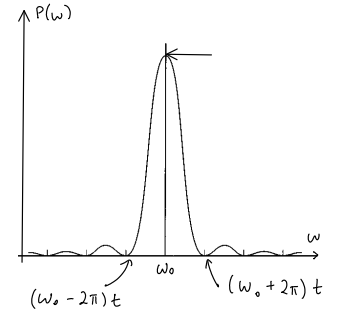
\includegraphics[width=0.7\textwidth]{Immagini/12_6/Pomega.PNG}
\caption{Grafico di $P_{if}(\omega)$\label{fig:P-omega}}
\end{figure}

\subsection{Fermi Golden Rule}
Estendiamo quanto appena visto al caso di uno spettro generale, sia discreto che continuo. Nello specifico, partiamo da $\ket{\varphi_i}$ autostato di $H_0$ nello spettro discreto, e vogliamo calcolare le $P_{if}$ con uno stato $\ket{f}=\ket{\alpha_f}$ nello spettro continuo.\\
Poiché per gli autostati del continuo vale la relazione di normalizzazione:
\begin{align*}
\braket{\alpha|\alpha'} = \delta(\alpha-\alpha')
\end{align*}
si ha che la probabilità di transizione ad un \textit{singolo specifico stato} è sempre nulla, visto che uno stato nel continuo ha \textit{misura nulla}.\\
Bisogna perciò considerare un \textbf{intervallo di stati}, che prendiamo \textit{vicini} allo stato $\alpha_F$ che ci interessa, ossia in un suo intorno $D_f$. Supponendo che tali possibili transizioni siano indipendenti tra loro, possiamo ottenere la $P_{if}$ integrando sul range dell'indice $\alpha \in D_f$ che identifica gli autoket:
\begin{align}
    P(\alpha_F,t) = \int_{\alpha \in D_f} |\braket{\alpha|\psi(t)}|^2 \, d\alpha
    \label{eqn:p-continue}
\end{align}
Poiché stiamo parlando di autoket di $H_0$, $\alpha$ è una funzione dell'autovalore $\mathcal{E}$, che possiamo usare perciò come indice per gli autoket. Differenziando otteniamo:
\begin{align*}
    \alpha = \alpha(\mathcal{E}) \Rightarrow d\alpha = \underbrace{\frac{d\alpha}{d\mathcal{E}}}_{\rho(\mathcal{E})} d\mathcal{E}
\end{align*}
dove $\rho(\mathcal{E})$ è la \textbf{densità di stati} (numero di stati per unità di energia) ad energia $\mathcal{E}$.\\

Più precisamente, ciò vale solo in assenza di degenerazione. Nel caso generale, per identificare un autoket di $H_0$ sono necessari due indici: $\alpha$ e l'\textit{indice di degenerazione} $\beta$. Ripetendo il passaggio precedente, giungeremo perciò a:
\begin{align*}
    d\alpha = \rho(\beta, \mathcal{E})\, d\mathcal{E}\,d\beta
\end{align*}
Sostituendo in (\ref{eqn:p-continue}) otteniamo:
\begin{align}
    P(\mathcal{E}_f,t) = \int_{\mathcal{E} \in \Delta\mathcal{E}} |\braket{\mathcal{E},\beta|\psi(t)}|^2 \rho(\mathcal{E},\beta)\, d\mathcal{E}
    \label{eqn:Pif-continue}
\end{align}
Al primo ordine, analogamente a quanto ricavato in (\ref{eqn:bn1}):
\begin{align*}
    \braket{\mathcal{E},\beta|\psi(t)} = \frac{1}{i\hbar} \int_0^t \exp(i\omega_{fi}\tau) \bra{\mathcal{E},\beta}W(\tau)\ket{\varphi_i} d\tau; \qquad \omega_{fi} = \frac{\mathcal{E}-\mathcal{E}_i}{\hbar}
\end{align*}

Calcoliamo esplicitamente la probabilità di transizione in due casi semplici. Per semplicità di notazione, lavoreremo nel caso nondegenere.
\begin{enumerate}
    \item \textbf{Potenziale costante} $W(t) \equiv W$. Questo è per esempio il caso di un potenziale che \q{si accende improvvisamente} a $t=0$. Si ha allora:
    \begin{align*}
        \braket{\mathcal{E}|\psi(t)} &= \frac{1}{i\hbar} \bra{\mathcal{E}}W\ket{\varphi_i} \int_0^t \exp(i\omega_{fi}\tau)d\tau =\\
        &= \frac{1}{i\hbar} \bra{\mathcal{E}}W\ket{\varphi_i} \frac{\exp(i\omega_{fi}t)-1}{i\omega_{fi}} =\\
        &= -\frac{1}{\hbar} \frac{\bra{\mathcal{E}}W\ket{\varphi_i}}{\omega_{fi}} \frac{\exp\left( \frac{i\omega_{fi}t}{2}\right) - \exp\left(-\frac{i\omega_{fi}t}{2}\right)}{\textcolor{Red}{2i}} \textcolor{Red}{2i} \exp\left( \frac{i\omega_{fi}t}{2}\right) =\\
        &= -\frac{\textcolor{Red}{2}i}{\hbar} \frac{\bra{\mathcal{E}}W\ket{\varphi_i}}{\omega_{fi}} \sin\left(\frac{\omega_{fi}t}{2}\right) \exp\left( \frac{i\omega_{fi}t}{2}\right)
    \end{align*}
    Prendendo il modulo quadro:
    \begin{align*}
       |\braket{\mathcal{E}|\psi(t)}|^2 = \frac{1}{\hbar^2} |\bra{\mathcal{E}}W\ket{\varphi_i}|^2 F\left(t, \frac{\mathcal{E}-\mathcal{E}_i}{\hbar}\right); \qquad F(t,\omega) = \left(\frac{\sin\left(\frac{\omega t}{2}\right)}{\frac{\omega}{\textcolor{Red}{2}}}\right)^2 
    \end{align*}
    Possiamo ora sostituire in (\ref{eqn:Pif-continue}), ottenendo:
    \begin{align*}
        P(\mathcal{E}_f,t) = \int_{\mathcal{E} \in \Delta \mathcal{E}} 
        \frac{1}{\hbar^2} |\bra{\mathcal{E}}W\ket{\varphi_i}|^2 F\left( t, \frac{\mathcal{E}-\mathcal{E}_i}{\hbar}\right) \rho(\mathcal{E}) d\mathcal{E}
    \end{align*}
    Sappiamo che $F$ è piccata attorno a $\mathcal{E}_i$, ed è tanto più stretta quanto più $t$ è grande. Supponendo allora che $t$ sia sufficientemente grande, si ha che $P(\mathcal{E}_f,t)$ è significativamente $\neq 0$ solo per $\mathcal{E}_f = \mathcal{E}_i$. Supponendo poi che $W$ e $\rho(\mathcal{E})$ siano \textit{approssimativamente costanti} in $\Delta\mathcal{E}$ (che pensiamo centrato in $\mathcal{E}_i$, per poter ottenere un risultato non $\approx 0$). Possiamo allora valutarli nel punto medio $\mathcal{E}_i$ e portarli fuori dall'integrale:
    \begin{align*}
        P(\mathcal{E}_f = \mathcal{E}_i, t) = \frac{1}{\hbar^2} |\bra{\mathcal{E}_i}W\ket{\varphi_i}|^2 \rho(\mathcal{E}_i) \int_{\mathcal{E}\in \Delta\mathcal{E}} F\left( t, \frac{\mathcal{E}-\mathcal{E}_i}{\hbar}\right)
    \end{align*}
    Con tali ipotesi, possiamo estendere il dominio di integrazione a tutto $\bb{R}$, dato che $F \approx 0$ per valori di poco diversi da $\mathcal{E}_i$. Così facendo possiamo calcolare l'integrale:
    \begin{align*}
        \int_{\bb{R}} \sin^2 \left( \frac{\omega_{fi}t}{2}\right) \frac{4}{\omega_{fi}^2}\,d\mathcal{E} = 4\hbar \int_{\bb{R}} \frac{1}{\omega^2_{fi}} \sin^2\left( \frac{\omega_{fi}t}{2}\right)\, d\omega_{fi}
    \end{align*}
    dove abbiamo usato il cambio di variabile:
    \begin{align*}
        \omega_{fi} = \frac{\mathcal{E}-\mathcal{E}_i}{\hbar} \Rightarrow d\omega_{fi} = \frac{d\mathcal{E}}{\hbar}
    \end{align*}
    Con un ulteriore cambio di variabile:
    \begin{align*}
        u = \frac{\omega_{fi}t}{2} \Rightarrow du = \frac{t}{2} d\omega_{fi}
    \end{align*}
    giungiamo infine a:
    \begin{align*}
        4\hbar \int_{\bb{R}} \frac{\sin^2(u)}{\frac{4u^2}{t^2}} \frac{2}{t} du = 2\hbar t \underbrace{\int_{\bb{R}} \frac{sin^2(u)}{u^2} du}_{=\pi} = 2\pi \hbar t
    \end{align*}
    E perciò la probabilità di transizione tra lo stato $\ket{\varphi_i}$ e lo stato $\ket{\alpha_F}$ di energia $\mathcal{E}(\alpha_F) = \mathcal{E}_i$ è data da:
    \begin{align*}
        P(\ket{\varphi_i} \to \ket{\alpha_f}, t) = \frac{2\pi t}{\hbar} |\bra{\alpha_f} W \ket{\varphi_i}|^2
    \end{align*}
    Tenendo conto anche della degenerazione si ottiene un'espressione leggermente più complessa:
    \begin{align*}
        dP(\ket{\varphi_i} \to \ket{\alpha_f},t) = d\beta \frac{2\pi t}{\hbar} |\bra{\alpha_f, \beta_f} W\ket{\varphi_i}|^2
    \end{align*}
    
    Definiamo infine il \textbf{rate} di transizione come la probabilità di transizione per unità di tempo:
    \begin{align*}
        w \equiv \frac{1}{t} P_{fi}(t)
    \end{align*}
    E giungiamo così alla regola d'oro di Fermi per perturbazioni costanti:
    \begin{align*}
        w = \frac{2\pi}{\hbar} |\bra{\alpha_f}W\ket{\varphi_i}|^2 \rho(\mathcal{E}_f); \qquad \mathcal{E}_f = \mathcal{E}_i
    \end{align*}
    
    \item \textbf{Perturbazione sinusoidale} $W(t) = W\sin(\omega t)$. Ripetendo tutti i passaggi del caso precedente, si giunge all'espressione (\textbf{regola d'oro di Fermi}):
    \begin{align*}
        w(\ket{\varphi_i}\to \ket{\alpha_f}) = \frac{2\pi}{\hbar} \rho(\beta_f,\mathcal{E}_f) |\bra{\beta_f, \mathcal{E}_f}W\ket{\varphi_i}|^2 \qquad \mathcal{E}_f = \mathcal{E}_i + \hbar \omega 
    \end{align*}
    che descrive il \textit{rate} di transizione per \textit{assorbimento} di radiazione. Nel caso di \textit{emissione} basta sostituire $\mathcal{E}_f = \mathcal{E}_i - \hbar \omega$.
\end{enumerate}


\begin{comment}
Ripetendo quanto visto prima nel caso di $W(t)\equiv W$ costante, si trova:
\begin{align*}
|\braket{\beta,\mathcal{E}|\psi(t)}|^2 = \frac{1}{\hbar^2} |\bra{\beta, \mathcal{E}}W \ket{\varphi_i}|^2 F\left(t, \frac{\mathcal{E}_f-\mathcal{E}_i}{\hbar}\right)
\end{align*}
dove il $\sin$ in $F$ converge (debolmente) per $t\to +\infty$ a:
\begin{align*}
\lim_{t\to +\infty} F\left(t, \frac{\mathcal{E}-\mathcal{E}_i}{\hbar}\right) = 2\pi \hbar t \delta(\mathcal{E}_f-\mathcal{E}_i) 
\end{align*}
Questo è un \textit{trucco matematico} che permette di risolvere facilmente l'integrazione (e si verifica sperimentalmente che il risultato è giusto, anche se richiederebbe una derivazione matematica più rigorosa, ma molto più complessa. Si intenda $t$ \q{sufficientemente alto}, ma non \q{troppo} in modo da non vanificare l'ipotesi di perturbazione).
Inserendo nella probabilità di transizione:
\begin{align*}
\delta P(\varphi_i, \alpha_t, t) = \delta \beta_f \frac{2\pi t}{\hbar} |\bra{\beta_f, \mathcal{E}_f = \mathcal{E}_i} W\ \ket{\varphi_i}|^2 
\end{align*}

D'altro canto, se poniamo $W(t) = W\sin(\omega t)$ si trova la \textit{Fermi Golden Rule}:
\begin{align*}
W(\varphi_i, \alpha_f) = \frac{d}{dt} \frac{\delta P}{\delta \beta} = \frac{\pi}{2\hbar} | \bra{\beta_f, \mathcal{E}_f = \mathcal{E}_i + \hbar \omega } W \ket{\varphi_i}|^2 \rho (\beta_f, \mathcal{E}_f = \mathcal{E}_i + \hbar \omega )
\end{align*}
dove abbiamo usato:
\begin{align*}
\int F(\beta) d\beta = d\beta F(\bar{\beta})
\end{align*}
\end{comment}


\chapter{Hardware quantistico}
Per realizzare nella pratica un computer quantistico è necessario soddisfare alcuni criteri, che furono formalizzati per la prima volta da Di Vincenzo nel 2000:
\begin{enumerate}
\item \textbf{Scalabilità}: qubit con una realizzazione ben definita e replicabile
\item \textbf{Reset}: possibilità di creare (stabilmente) stati $\ket{00000\dots 0}$
\item \textbf{Tempi di coerenza lunghi} rispetto alla durata di esecuzione - e perciò ben più lunghi della durata di un gate.\\
Detto cioè $\tau_d$ il \textit{rate} di decoerenza, e $\tau_g$ la durata media necessaria per effettuare un'operazione (\textit{gate time}, equivalente al \textit{clock} di un computer classico), vorremmo che $\tau_d/\tau_g \gg 1$. Nello specifico, sarebbe un buon risultato avere $\tau_d/\tau_g > 10^4$ - dato che ciò permetterebbe di realizzare anche gli algoritmi di \textit{error-correction}.
\item \textbf{Set universale di gate}
\item \textbf{Read-out efficiente}, ossia possibilità di misurare gli stati prodotti dal computer quantistico in maniera affidabile
\end{enumerate}

Negli ultimi decenni si sono esaminati diversi sistemi hardware per cercare di raggiungere tali obiettivi. I principali sono:
\begin{itemize}
\item Cavity QED
\item Solid-state devices (quantum dot, circuiti in grado di \textit{intrappolare} singoli elettroni)
\item Atomi freddi
\item Ioni intrappolati
\item Circuiti superconduttivi
\end{itemize}

I più promettenti sono gli ultimi due, che ora introdurremo.

\subsection{Ioni intrappolati}
In questa implementazione fisica, i qubit sono dati da \textit{ioni}, che vengono confinati grazie ad una \textit{Paul trap}, mediante un campo elettrico.

\begin{figure}[H]
\centering
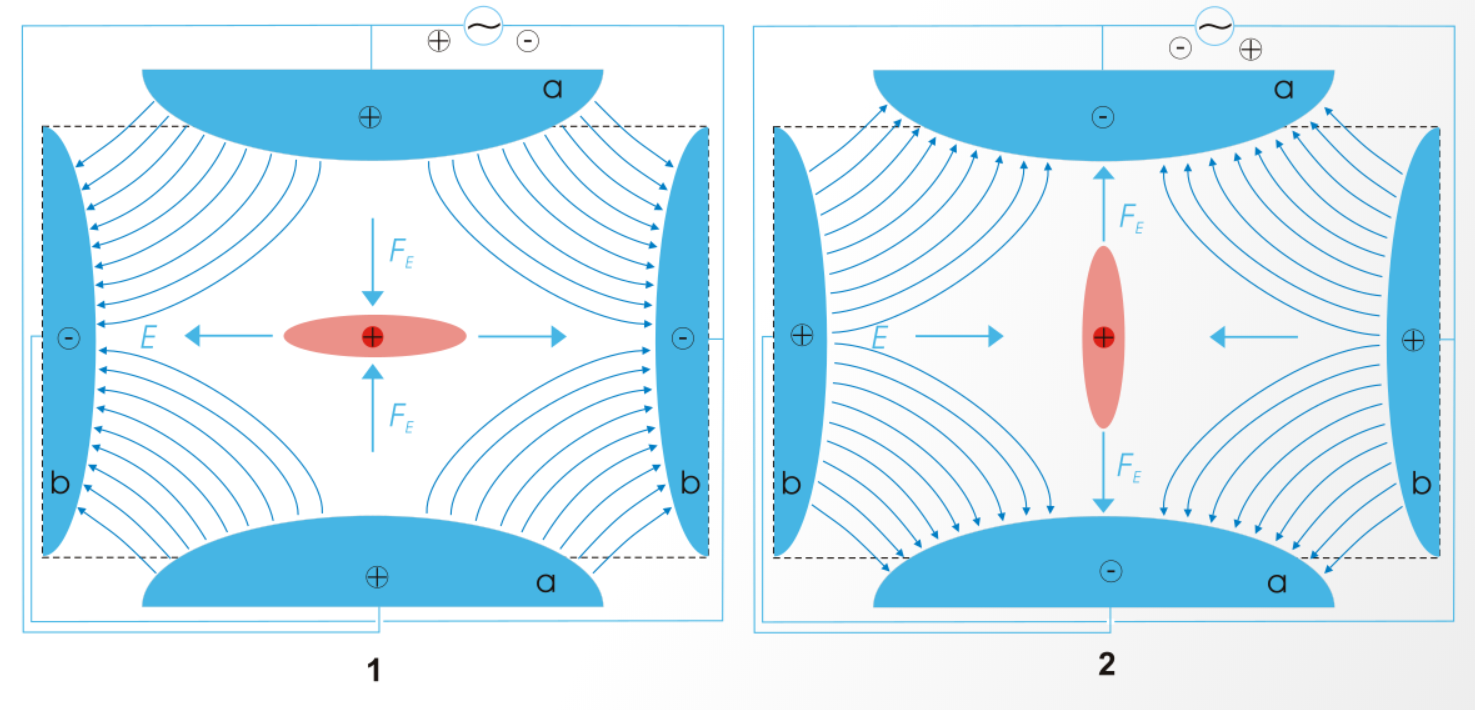
\includegraphics[width=0.8\textwidth]{Immagini/12_6/paul_trap.PNG}
\caption{Schema di una Paul trap. Uno ione positivo è sospeso tra coppie di elettrodi, che esercitano forze repulsive o attrattive in maniera periodica.\label{fig:Paul-trap}}
\end{figure}

Non è possibile realizzare una trappola per soli effetti elettrostatici (teorema di Earnshaw), e perciò è necessario introdurre \textit{correnti} e \textit{scambiare periodicamente le cariche} sugli elettrodi, ad una frequenza sufficientemente alta (figura \ref{fig:Paul-trap}).\\
A livello fisico, perciò, lo ione può essere considerato come un oscillatore armonico in $d=3$, con pulsazioni $\omega_z$, $\omega_x$ e $\omega_y$. Due di queste sono fissate \q{in modo stretto} dalla trappola, e l'altra viene utilizzata come grado di libertà quantistico. In altre parole: è richiesta molta energia per eccitare i modi lungo $x$ o $y$, e molta meno per quelli lungo $z$ - che quindi sono quelli effettivamente raggiunti.\\

Consideriamo perciò $N$ ioni nella stessa trappola, per cui si ha l'Hamiltoniana:
\begin{align*}
H = \sum_{i=1}^N \frac{p_i^2}{2m} + \sum_{i=1}^N \frac{1}{2}\omega_z^2 z_i^2 + \sum_{i=1}^N \sum_{j>i} \frac{q^2}{4\pi\epsilon_0|r_i-r_j|}
\end{align*}

Tale hamiltoniana si risolve con i procedimenti utilizzati per gli oscillatori armonici accoppiati. In particolare ne consideriamo i \textit{modi normali di oscillazione} - e in particolare i due in cui $N$ particelle che oscillano \q{in fase} o \q{in opposizione di fase}.\\
Lo stato del sistema è allora dato da:
\begin{align*}
\ket{\alpha_1}\ket{\alpha_2} \dots \ket{\alpha_N} \ket{n}
\end{align*}
dove $\ket{\alpha_i}$ sono stati interni agli ioni (es. due livelli energetici ben conosciuti) e $\ket{n}$ quelli dell'oscillatore armonico lungo $z$. In ordine di energia avremo allora:
\begin{align*}
\ket{g,0},\ket{g,1},\ket{g,2} \dots \ket{e,0},\ket{e,1},\ket{e,2},\dots
\end{align*}
(dove si sottintende il prodotto tensore con $\ket{0}_x\ket{0}_y$ che indica lo stato fondamentale degli oscillatori lungo $x$ e $y$)
dove con $g$ indichiamo lo stato fondamentale e con $e$ il primo eccitato. Utilizzando \textit{laser} possiamo stimolare delle transizioni tra i vari livelli.\\
Il reset avviene eccitando le transizioni $\ket{g,n}\to \ket{e,n-1}$. A tal punto uno ione eccitato \textit{tende} a decadere nello stato fondamentale, e quindi $\ket{e,n-1}\to \ket{g,n-1}$. Poiché tali transizioni hanno tutte la stessa pulsazione $\omega$ (per effetto degli autovalori di un oscillatore armonico) si può usare un unico laser per \textit{portare i qubit tutti allo stato fondamentale}. Tale procedimento è detto \textbf{side-band cooling}. Ciò ha un'efficienza $P>99.9\%$.\\
Utilizzando poi \textit{due laser} indipendenti è possibile realizzare il \textit{Cirac-Zoller Gate}. 

\begin{figure}[H]
\centering
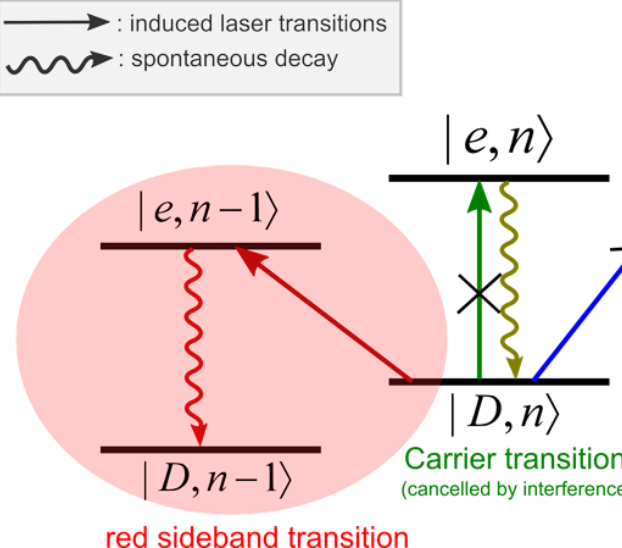
\includegraphics[width=0.7\textwidth]{Immagini/12_6/sideband.PNG}
\caption{Schema del procedimento di side-band cooling\label{fig:sideband-cooling}}
\end{figure}

\subsection{Superconducting qubit} \marginpar{\danger Parte da ricontrollare}
Raffreddando alcuni materiali si creano naturalmente \textit{coppie di Cooper}, ossia coppie di elettroni \q{entangled}, che si comportano \q{come un bosone} e possono condensare\footnote{L'entanglement in realtà avviene nello spazio reciproco, non in quello diretto - e quindi si ha una \textit{trasformata di Fourier}. Tutto ciò si tratta nel framework della \textit{seconda quantizzazione}, che è oltre agli obiettivi di questo corso.}. Tali coppie possono muoversi \q{senza resistenza}, e quindi produrre \q{correnti che non decadono} - nel fenomeno della \textbf{superconduttività}.\\

Per realizzare i qubit si usano delle \textbf{giunzioni Josephson}, realizzate inserendo un sottile strato isolante tra due strati di superconduttore - che si comportano come un condensatore con capacità $C_j$. Le coppie di Cooper possono \textit{passare attraverso la barriera} per effetto tunnel. Connettendo una giunzione Josephson a un condensatore $C_\gamma$ si crea un \textbf{charge qubit}. Le coppie di Cooper non possono attraversare le armature del condensatore (la distanza è troppo ampia) - e perciò lo stato superconduttore che si affaccia al condensatore è \q{un'isola}, nel senso che è completamente scollegato dal resto del circuito - e per depositarvi una coppia è necessario spendere una certa energia.\\
L'Hamiltoniana di tale sistema si dimostra essere:
\begin{align*}
H = \mathcal{E}_c (n-n_g)^2 - \mathcal{E}_j \cos\phi \qquad [n,\phi]=i
\end{align*}
dove $n$ è il numero di coppie che occupano l'isola, e $n_g = C_\gamma V/(2e)$ è un numero \q{base} di coppie (corrispondente allo \q{zero dell'energia}), fissato dal potenziale $V$ che alimenta il circuito. Si trova poi $\mathcal{E}_c = (2e)^2/(2(C_j+C_\gamma))$. $\phi = i\partial_n$ è il secondo numero quantico importante per il sistema, ed è detto \textit{fase del superconduttore}.\\
Detto $\ket{n}$ lo stato in cui vi sono $n$ coppie nell'isola si ha:
\begin{align*}
H = \mathcal{E}_c \sum (n-n_g)^2 \ket{n}\bra{n} - \frac{1}{2}\mathcal{E}_j \sum \ket{n+1}\bra{n} + \ket{n}\bra{n+1}
\end{align*} 

Graficando i livelli energetici $\mathcal{E}$ in funzione di $n_g$ si ottiene:
\begin{figure}[H]
\centering
[Missing]
\caption{Grafico dei livelli\label{?}}
\end{figure}

La presenza dei termini di interazione ($\cos\phi$) fa sì che i tratti del grafico di $\mathcal{E}$ non si intersechino tra loro (\textit{avoided crossing}). Si realizzano allora livelli separati che possono essere usati come qubit.

\end{document}

